\documentclass[11pt,a4paper]{article}

% =================================================
% PACKAGES
% =================================================

\usepackage[a4paper,left=2.0cm,right=2.0cm,top=1.55cm,bottom=1.55cm]{geometry}
\usepackage[T1]{fontenc}
\usepackage{lmodern}
\usepackage{graphicx}
\usepackage{xcolor}
\usepackage{array}
\usepackage{tabularx}
\usepackage{ragged2e}
\usepackage{enumitem}
\usepackage{fancyhdr}
\usepackage{tikz}
\usepackage{amssymb}
\usepackage{float}
\usepackage{needspace}

% =================================================
% COLOR
% =================================================

\definecolor{TitleBlue}{RGB}{61,103,154}

% =================================================
% GENERAL SETTINGS
% =================================================

\setlength{\parindent}{0pt}
\setlength{\parskip}{4pt}

\renewcommand{\arraystretch}{1.15}

\setlist[itemize]{
    leftmargin=5mm,
    itemsep=2pt,
    topsep=2pt
}

\setlist[enumerate]{
    leftmargin=6mm,
    itemsep=2pt,
    topsep=2pt
}

% =================================================
% CUSTOM HEADINGS
% =================================================

\newcommand{\blueheading}[1]{%
    \needspace{7\baselineskip}
    {\sffamily
    \color{TitleBlue}
    \fontsize{15}{18}
    \selectfont
    #1}%
}

\newcommand{\bluebigheading}[1]{%
    {\sffamily
    \bfseries
    \color{TitleBlue}
    \fontsize{16}{19}
    \selectfont
    #1}%
}

\newcommand{\instruction}[1]{%
    {\itshape
    \fontsize{10.5}{12.5}
    \selectfont
    #1}%
}

% =================================================
% ANSWER BOX
% =================================================

\newcommand{\answerbox}[1]{%
    \vspace{3pt}
    \noindent
    \fbox{%
        \begin{minipage}{%
            \dimexpr\textwidth-2\fboxsep-2\fboxrule\relax
        }
        \vspace{2mm}
        #1
        \vspace{2mm}
        \end{minipage}%
    }
    \vspace{3pt}
}

% =================================================
% PHOTO BOX
% =================================================

\newcommand{\photobox}[1]{%
    \fbox{%
        \includegraphics[
            width=2.8cm,
            height=3.4cm
        ]{#1}%
    }%
}

% =================================================
% SECTION BLOCK
% Keeps heading with its following content
% =================================================

\newenvironment{sectionblock}
{%
    \par
    \needspace{8\baselineskip}
}
{%
    \par
}

% =================================================
% HEADER AND FOOTER
% =================================================

\pagestyle{fancy}

\fancyhf{}

\renewcommand{\headrulewidth}{0pt}
\renewcommand{\footrulewidth}{0pt}

\fancyhead[L]{%
    \sffamily
    \bfseries
    \itshape
    \fontsize{10.5}{12}
    \selectfont
    DSCPP-III-2026-T307
}

\fancyhead[R]{%
    \sffamily
    \bfseries
    \fontsize{10.5}{12}
    \selectfont
    PROJECT PROPOSAL
}

\fancyfoot[R]{%
    \itshape
    \fontsize{10}{12}
    \selectfont
    Page \thepage
}

\setlength{\headheight}{14pt}
\setlength{\headsep}{23pt}
\setlength{\footskip}{24pt}

% =================================================
% DOCUMENT
% =================================================

\begin{document}

% =================================================
% PAGE 1
% =================================================

\vspace*{4mm}

\bluebigheading{PROJECT AND TEAM INFORMATION}

\vspace{12mm}

% -------------------------------------------------
% PROJECT TITLE
% -------------------------------------------------

\begin{sectionblock}

\blueheading{Project Title}

\vspace{1mm}

\instruction{
(Try to choose a catchy title. Max 20 words).
}

\answerbox{
\textbf{
Smart Student Life: A Campus Assistant for Academic and College Activity Management
}
}

\end{sectionblock}

\vspace{7mm}

% -------------------------------------------------
% STUDENT / TEAM INFORMATION
% -------------------------------------------------

\begin{sectionblock}

\blueheading{Student / Team Information}

\vspace{2mm}

\noindent
\begin{tabularx}{\textwidth}{
    |>{\RaggedRight\arraybackslash}p{0.66\textwidth}
    |>{\RaggedRight\arraybackslash}X|
}
\hline

% =================================================
% TEAM NAME
% =================================================

\begin{minipage}[t]{\linewidth}
\vspace{2mm}

\textit{Team Name:}

Smart Campus Assistant

\vspace{2mm}
\end{minipage}
&
\begin{minipage}[t]{\linewidth}
\vspace{2mm}

\textit{Team Number:}

\textit{__________}

\vspace{2mm}
\end{minipage}
\\
\hline

% =================================================
% MEMBER 1
% =================================================

\begin{minipage}[t]{\linewidth}
\vspace{2mm}

\textbf{Team Member 1 -- Team Lead}

\textit{Solanki, Anshuman}

\textit{Student ID: 2512510022}

\textit{Email: 2512510022@geu.ac.in}

\vspace{2mm}
\end{minipage}
&
\begin{minipage}[t]{\linewidth}
\vspace{2mm}

\begin{center}
\textit{Photo}

\vspace{2mm}

\photobox{member1.png}
\end{center}

\vspace{1mm}
\end{minipage}
\\
\hline

% =================================================
% MEMBER 2
% =================================================

\begin{minipage}[t]{\linewidth}
\vspace{2mm}

\textbf{Team Member 2}

\textit{Mundepi, Arush}

\textit{Student ID: 2510370121}

\textit{Email: 2510370121@geu.ac.in}

\vspace{2mm}
\end{minipage}
&
\begin{minipage}[t]{\linewidth}
\vspace{2mm}

\begin{center}
\textit{Photo}

\vspace{2mm}

\photobox{member2.png}
\end{center}

\vspace{1mm}
\end{minipage}
\\
\hline

% =================================================
% MEMBER 3
% =================================================

\begin{minipage}[t]{\linewidth}
\vspace{2mm}

\textbf{Team Member 3}

\textit{Singh, Anubhav}

\textit{Student ID: 2510370452}

\textit{Email: 2510370452@geu.ac.in}

\vspace{2mm}
\end{minipage}
&
\begin{minipage}[t]{\linewidth}
\vspace{2mm}

\begin{center}
\textit{Photo}

\vspace{2mm}

\photobox{member3.png}
\end{center}

\vspace{1mm}
\end{minipage}
\\
\hline

\end{tabularx}

\end{sectionblock}

\newpage

% =================================================
% PAGE 2
% PROPOSAL DESCRIPTION
% =================================================

\bluebigheading{PROPOSAL DESCRIPTION (10 pts)}

\vspace{10mm}

% =================================================
% MOTIVATION
% =================================================

\begin{sectionblock}

\blueheading{Motivation (1 pt)}

\vspace{1mm}

\instruction{
(Describe the problem you want to solve and why it is important. Max 300 words).
}

\answerbox{

Students have to manage several academic and campus-related activities such as assignments, examinations, attendance, library work, college events, and placement opportunities. These activities are often tracked using different notebooks, calendars, applications, or informal reminders, which can make it difficult to maintain a clear overview of pending work.

The proposed Smart Student Life / Campus Assistant provides a single console-based system where students can organize and manage these activities efficiently. The main challenge addressed by the project is not only storing tasks but also identifying which task requires immediate attention.

To solve this problem, the system introduces a deadline-based priority mechanism. Whenever a student enters a task along with its due date, the application compares the due date with the current system date and assigns an appropriate priority. A Priority Queue is then used to arrange tasks so that more urgent activities are displayed first.

The project combines practical student activity management with important Data Structures and programming concepts. It aims to help students organize their college responsibilities in a simple, systematic, and efficient manner.

}

\end{sectionblock}

\vspace{6mm}

% =================================================
% STATE OF THE ART
% =================================================

\begin{sectionblock}

\blueheading{State of the Art / Existing Solution (1 pt)}

\vspace{1mm}

\instruction{
(Describe existing solutions and their limitations. Max 300 words).
}

\answerbox{

Students commonly use separate tools such as notebooks, mobile reminder applications, calendars, spreadsheets, or learning-management systems to keep track of academic activities. These solutions can be useful for individual purposes, but information may remain distributed across different platforms.

Most basic task-management systems allow users to create tasks and assign dates, but they may not specifically focus on the combination of academic and campus activities. They also may not demonstrate how fundamental data structures can be used to organize and prioritize such information.

The proposed system addresses these limitations by bringing assignments, examinations, attendance, library activities, college events, and placement opportunities into one application. It additionally provides an automatic deadline-based priority mechanism. The system compares a task's due date with the current system date and assigns a priority level. A Priority Queue is then used to present urgent tasks before less urgent tasks.

Therefore, the project provides both a practical student-management solution and an academic demonstration of data structures, object-oriented programming, and file handling.

}

\end{sectionblock}

\vspace{6mm}

% =================================================
% PROJECT GOALS AND MILESTONES
% =================================================

\begin{sectionblock}

\blueheading{Project Goals and Milestones (2 pts)}

\vspace{1mm}

\instruction{
(List the major goals of the project and the milestones planned to achieve them).
}

\answerbox{

\textbf{Major Goals}

\begin{itemize}

    \item Develop a console-based Smart Student Life / Campus Assistant.

    \item Provide modules for student profile and campus activities.

    \item Manage assignments and examination-related tasks.

    \item Maintain attendance-related information.

    \item Provide library and college-event management features.

    \item Maintain placement opportunities and related information.

    \item Implement automatic deadline-based task prioritization.

    \item Use a Priority Queue to display urgent tasks first.

    \item Compare task due dates with the current system date.

    \item Demonstrate Linked List, Queue, Priority Queue, Stack, and BST.

    \item Demonstrate C++ OOP concepts including classes, objects, encapsulation, inheritance, and polymorphism.

    \item Use file handling for permanent storage of information.

\end{itemize}

\textbf{Planned Milestones}

\begin{enumerate}

    \item Requirement analysis and system design.

    \item Design of data structures and module organization.

    \item Development of student profile and activity modules.

    \item Implementation of assignment, exam, attendance, library, event, and placement modules.

    \item Implementation of deadline comparison and priority assignment.

    \item Integration of Priority Queue and other required data structures.

    \item Implementation of OOP concepts and file handling.

    \item Testing, debugging, integration, and final demonstration.

\end{enumerate}

}

\end{sectionblock}

\newpage

% =================================================
% PAGE 3
% PROJECT APPROACH
% =================================================

\begin{sectionblock}

\blueheading{Project Approach (2 pts)}

\vspace{1mm}

\instruction{
(Explain the approach, technologies, algorithms, and data structures that will be used).
}

\answerbox{

The project will be developed as a console-based application using C and C++. The system will be divided into modules so that different academic and campus activities can be managed independently while remaining part of a single application.

\textbf{Programming Languages}

C will be used for implementing and demonstrating fundamental data structures, while C++ will be used to demonstrate object-oriented programming concepts and integrate the overall application.

\textbf{Data Structures}

\begin{itemize}

    \item \textbf{Linked List:}
    Used for maintaining dynamic collections of records where the number of elements can change.

    \item \textbf{Queue:}
    Used for activities where information needs to be processed in first-in-first-out order.

    \item \textbf{Priority Queue:}
    Used for arranging tasks according to their urgency and deadlines.

    \item \textbf{Stack:}
    Used where last-in-first-out processing is suitable, such as maintaining recent actions.

    \item \textbf{Binary Search Tree (BST):}
    Used for organized searching and storing records based on a key.

\end{itemize}

\textbf{Priority Mechanism}

When a student enters a task, its title, category, and due date are stored. The program obtains the current system date and calculates the difference between the current date and the task deadline. Based on the remaining time, the task is assigned a priority level. Tasks with nearer deadlines receive higher priority and are placed ahead of less urgent tasks in the Priority Queue.

\textbf{Object-Oriented Programming}

Classes and objects will represent entities such as Student, Assignment, Exam, Event, Library Record, and Placement Opportunity. Encapsulation will keep related data and functions together. Inheritance and polymorphism will be used where common properties and behaviours can be shared among different types of activities.

\textbf{File Handling}

File handling will be used to store records permanently. This ensures that student information and activity data remain available even after the application is closed and reopened.

}

\end{sectionblock}

\vspace{6mm}

% =================================================
% SYSTEM ARCHITECTURE
% =================================================

\begin{sectionblock}

\blueheading{System Architecture / High-Level Design (1 pt)}

\vspace{1mm}

\instruction{
(Show the major modules and the flow of information in the proposed system).
}

\answerbox{

\begin{center}

\resizebox{0.88\textwidth}{!}{%
\begin{tikzpicture}[
    box/.style={
        draw,
        rounded corners,
        align=center,
        text width=3.4cm,
        minimum height=0.85cm,
        inner sep=5pt
    },
    arrow/.style={
        ->,
        >=stealth,
        thick
    }
]

\node[box] (student) at (0,0)
{
    Student
};

\node[box] (menu) at (0,-1.7)
{
    Main Menu /\\
    Console Interface
};

\node[box] (academic) at (-3.8,-3.5)
{
    Academic Modules\\
    Assignments\\
    Exams\\
    Attendance
};

\node[box] (campus) at (3.8,-3.5)
{
    Campus Modules\\
    Library\\
    Events\\
    Placements
};

\node[box] (priority) at (0,-5.5)
{
    Deadline Analysis\\
    Current System Date\\
    Priority Assignment
};

\node[box] (pq) at (0,-7.4)
{
    Priority Queue\\
    Urgent Tasks First
};

\node[box] (ds) at (-3.8,-9.5)
{
    Data Structures\\
    Linked List\\
    Queue / Stack / BST
};

\node[box] (file) at (3.8,-9.5)
{
    File Handling\\
    Permanent Storage
};

\draw[arrow] (student) -- (menu);

\draw[arrow] (menu) -- (academic);
\draw[arrow] (menu) -- (campus);

\draw[arrow] (academic) -- (priority);
\draw[arrow] (campus) -- (priority);

\draw[arrow] (priority) -- (pq);

\draw[arrow] (pq) -- (ds);
\draw[arrow] (pq) -- (file);

\end{tikzpicture}%
}

\vspace{4mm}

The student interacts with the console interface through the main menu. Academic and campus modules collect the required information. Deadline-based tasks are processed through the priority mechanism, while the required data structures and file handling provide efficient organization and permanent storage.

\end{center}

}

\end{sectionblock}

\newpage

% =================================================
% PAGE 4
% PROJECT OUTCOME
% =================================================

\begin{sectionblock}

\blueheading{Project Outcome / Deliverables (1 pt)}

\vspace{1mm}

\instruction{
(Describe what will be delivered at the end of the project).
}

\answerbox{

At the end of the project, a functional console-based Smart Student Life / Campus Assistant will be delivered.

The major deliverables will include:

\begin{itemize}

    \item A student profile management module.

    \item Assignment management with task deadlines.

    \item Examination management.

    \item Attendance information management.

    \item Library activity management.

    \item College event management.

    \item Placement opportunity management.

    \item Automatic deadline-based priority assignment.

    \item Priority Queue based display of urgent tasks.

    \item Current system date comparison for deadline evaluation.

    \item Implementation of Linked List, Queue, Priority Queue, Stack, and BST.

    \item Implementation of C++ classes, objects, encapsulation, inheritance, and polymorphism.

    \item File handling for permanent storage.

    \item A tested and integrated console application demonstrating all major features.

\end{itemize}

The final system will provide students with an organized way to manage their college responsibilities while demonstrating the practical application of Data Structures, OOP, algorithms, and file handling.

}

\end{sectionblock}

\vspace{6mm}

% =================================================
% ASSUMPTIONS AND CONSTRAINTS
% =================================================

\begin{sectionblock}

\blueheading{Assumptions and Constraints (1 pt)}

\vspace{1mm}

\instruction{
(List important assumptions, constraints, and limitations of the proposed system).
}

\answerbox{

\textbf{Assumptions}

\begin{itemize}

    \item The application will primarily be operated through a console interface.

    \item Students will enter correct and meaningful information.

    \item Task deadlines will be entered using a valid date format.

    \item The system date will be obtained from the computer's operating system.

    \item The application will have permission to read and write its required data files.

\end{itemize}

\textbf{Constraints}

\begin{itemize}

    \item The first version is intended as a console-based application.

    \item The system does not depend on an internet connection for basic task management.

    \item Data persistence will be implemented through local file handling.

    \item The priority mechanism depends on the correctness of the entered deadline.

    \item The project focuses on demonstrating academic and campus activity management rather than replacing complete institutional systems.

\end{itemize}

}

\end{sectionblock}

\vspace{6mm}

% =================================================
% REFERENCES
% =================================================

\begin{sectionblock}

\blueheading{References}

\vspace{2mm}

\answerbox{

\begin{enumerate}

    \item Brian W. Kernighan and Dennis M. Ritchie,
    \textit{The C Programming Language},
    Prentice Hall.

    \item Bjarne Stroustrup,
    \textit{The C++ Programming Language},
    Addison-Wesley.

    \item Ellis Horowitz, Sartaj Sahni, and Susan Anderson-Freed,
    \textit{Fundamentals of Data Structures in C},
    Computer Science Press.

    \item Thomas H. Cormen, Charles E. Leiserson, Ronald L. Rivest, and Clifford Stein,
    \textit{Introduction to Algorithms},
    MIT Press.

    \item Standard C++ documentation and references for object-oriented programming, STL containers, queues, priority queues, and file streams.

\end{enumerate}

}

\end{sectionblock}

\vfill

\begin{center}

\textit{
\small
Smart Student Life / Campus Assistant -- Phase-I Project Synopsis
}

\end{center}

% =================================================
% END DOCUMENT
% =================================================

\end{document}